% =============================================================================
% Project : THE_PHILOSOPHY_OF_VIABILITY
% Book    : Book I — Ontology of Viability
% Book ID : VS.B01
%
% File    : 4_ASSETS/illustrations/VS.B01.P01.C03.S08.SS08.P003.IL01.manifestation_plurality_and_identity_scope.tex
%
% Asset:
%   Illustration IL01 — Manifestation Plurality and Identity Scope
%
% Purpose :
%   To illustrate that multiple manifestations can be distinguished
%   without deciding, solely on that basis, whether one or multiple
%   identities are involved.
%
% =============================================================================

\begin{figure}[htbp]
\centering

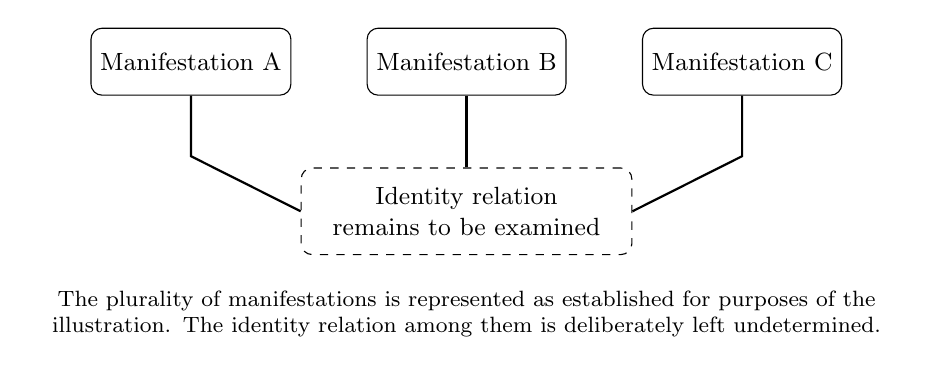
\begin{tikzpicture}[
    manifestation/.style={
        draw,
        rounded corners,
        minimum width=2.1cm,
        minimum height=0.85cm,
        align=center,
        font=\small
    },
    question/.style={
        draw,
        rounded corners,
        dashed,
        minimum width=4.2cm,
        minimum height=1.1cm,
        align=center,
        font=\small
    },
    relation/.style={
        thick,
        -
    }
]

\node[manifestation] (m1) at (-3.5,1.5) {Manifestation A};
\node[manifestation] (m2) at (0,1.5) {Manifestation B};
\node[manifestation] (m3) at (3.5,1.5) {Manifestation C};

\node[question] (identity) at (0,-0.4) {
    Identity relation\\
    remains to be examined
};

\draw[relation] (m1.south) -- (-3.5,0.3) -- (identity.west);
\draw[relation] (m2.south) -- (identity.north);
\draw[relation] (m3.south) -- (3.5,0.3) -- (identity.east);

\node[
    align=center,
    text width=0.9\textwidth,
    font=\footnotesize
] at (0,-1.7) {
    The plurality of manifestations is represented as established
    for purposes of the illustration. The identity relation among
    them is deliberately left undetermined.
};

\end{tikzpicture}

\caption{Plurality of Manifestations and the Unresolved Identity Relation}
\label{fig:manifestation-plurality-and-identity-scope}
\end{figure}

% =============================================================================
% END OF ILLUSTRATION IL01
% =============================================================================